% 导言区,进行全局设置
\documentclass[12pt]{ctexart}%book, report, latter, 引入文档类

%\usepackage{ctex}
%\usepackage[fleqn]{amsmath}
\usepackage{amsmath}
\usepackage{amssymb}
\usepackage{fancyhdr}
\usepackage{lastpage}
\usepackage{graphicx}
\usepackage{float}
\usepackage[colorlinks,linkcolor=black]{hyperref} % set super link

\usepackage{geometry}
\geometry{a4paper,top=2.54cm,left=3.18cm,bottom=2.54cm,right=3.18cm,includehead,includefoot}

% \newcommand命令的定义,新的命令
\newcommand\degree{^\circ}
\title{\kaishu Linear Model}
\author{Fish}
\date{\today}

% 内容与格式分离
% 设置标题的格式
\ctexset {
	section = {
		format+=\zihao {-4} \heiti \raggedright,
		name = {,},
		%number = \chinese{section},
		beforeskip = 1.0ex plus 0.2ex minus .2ex,
		afterskip = 1.0ex plus 0.2ex minus .2ex,
		aftername = \hspace{0pt}
	},
	subsection = {
		format+=\zihao{5} \heiti \raggedright,
		% name={\thesubsection},
		name = {,},
		%number = \arabic{subsection},
		beforeskip = 1.0ex plus 0.2ex minus .2ex,
		afterskip = 1.0ex plus 0.2ex minus .2ex,
		aftername = \hspace{0pt}
	}
}

% 正文区(文稿区),有且只有一个document环境
% \begim{*环境名称}
%        内容
% \end{*环境名称}
\begin{document}
	\maketitle
	
	%\clearpage
	\renewcommand{\contentsname}{Content} % set the 目录 to Content
	\tableofcontents
	\clearpage
	\pagestyle{fancy}
	\lhead{linear model by wzs}                   
	\rhead{Page \thepage{} of \pageref{LastPage}}
	\setcounter{page}{1}
	
	\section{\quad What}
	{\heiti \zihao{4}define the example x described by d property, $x=(x_1; x_2;...; x_d)$, among the variable x, $x_i$ is decided by ith property of x.}
	
	linear model showed as follow:
	\begin{equation}
		f(x)={{w}_{1}}{{x}_{1}}+{{w}_{2}}{{x}_{2}}+...+{{w}_{d}}{{x}_{d}}+b
	\end{equation}
		whether x has d property
		
	vector as well:
	\begin{eqnarray}
	f(x)={{w}^{T}}x+b
	\end{eqnarray}
%%%%%%%%%%%%%%%%%%%%%%%%%%%%%%%%%%%%%%%%%%%%%%%%%%%%%%%%%%%%%%%%%%%%%%%%%%%%%%%%%%%%%%%%%%%%%%%
%%%%%%%%%%%%%%%%%%%%%%%%%%%%%%%%%%%%%%%%%%%%%%%%%%%%%%%%%%%%%%%%%%%%%%%%%%%%%%%%%%%%%%%%%%%%%%%
	\section{\quad one sample has one property}
	{\heiti \zihao{4} to simplify the situation, we assump that the input x propert has only one.}
	
	\subsection{\quad background}
	we have dataset: $D = {(x_1, y_1)),(x_2, y_2),...,(x_m, y_m)}$, to study a model predict tab of output more correctly.
	
	\subsection{\quad analysis}
	to study model: $f(x)={{w}^{T}}x+b$, make the predict result $f(x_i)\cong y_i$, the $w, b$ need to be known.
	
	{\heiti mean square error} is correspondinng to {\heiti Euclidean distance}.  The way solve model based on mean square error named least square method. according to linear regression, least square method try to find a line that make the Euclidean distance sum of sample to line be least.
	
	\subsection{\quad processing}
		find least value of equation 3 and 4, get the $w^*,b^*$ 
		%\setlength{\abovedisplayskip}{1pt}
		\begin{align}
			({{w}^{*}},{{b}^{*}}) & =\underset{(w,b)}{\mathop{\arg \min }}\,\sum\limits_{i=1}^{m}{{{(f({{x}_{i}})-{{y}_{i}})}^{2}}} \\ 
			& =\underset{(w,b)}{\mathop{\arg \min }}\,\sum\limits_{i=1}^{m}{{{(w{{x}_{i}}+b-{{y}_{i}})}^{2}}} 
		\end{align}
		the progress solving the above equation named least square parameter estimation. there differenetiate w and b, could get following part:
		\begin{align}
			\frac{\partial E(w,b)}{\partial w}&=\sum\limits_{i=1}^{m}{2(-{{y}_{i}}+b+w{{x}_{i}}){{x}_{i}}}=2\sum\limits_{i=1}^{m}{[wx_{i}^{2}-({{y}_{i}}-b)}{{x}_{i}}]\\
			\frac{\partial E(w,b)}{\partial b}&=\sum\limits_{i=1}^{m}{2(-{{y}_{i}}+b+w{{x}_{i}})}=2[mb-\sum\limits_{i=1}^{m}{({{y}_{i}}-w{{x}_{i}}})]
		\end{align}

		then optimizer solution fo closed-form is shown:
		\begin{align}
			w&=\frac{\sum\limits_{i=1}^{m}{{{y}_{i}}({{x}_{i}}-\bar{x})}}{\sum\limits_{i=1}^{m}{x_{i}^{2}-\frac{1}{m}{{(\sum\limits_{i=1}^{m}{{{x}_{i}}})}^{2}}}}\\
			b&=\frac{1}{m}\sum\limits_{i=1}^{m}{(y{}_{i}-w{{x}_{i}})}
		\end{align}
%%%%%%%%%%%%%%%%%%%%%%%%%%%%%%%%%%%%%%%%%%%%%%%%%%%%%%%%%%%%%%%%%%%%%%%%%%%%%%%%%%%%%%%%%%%%%%%
%%%%%%%%%%%%%%%%%%%%%%%%%%%%%%%%%%%%%%%%%%%%%%%%%%%%%%%%%%%%%%%%%%%%%%%%%%%%%%%%%%%%%%%%%%%%%%%
	\section{\quad one sample has multiply property}
		\begin{figure}[H]
			\centering
			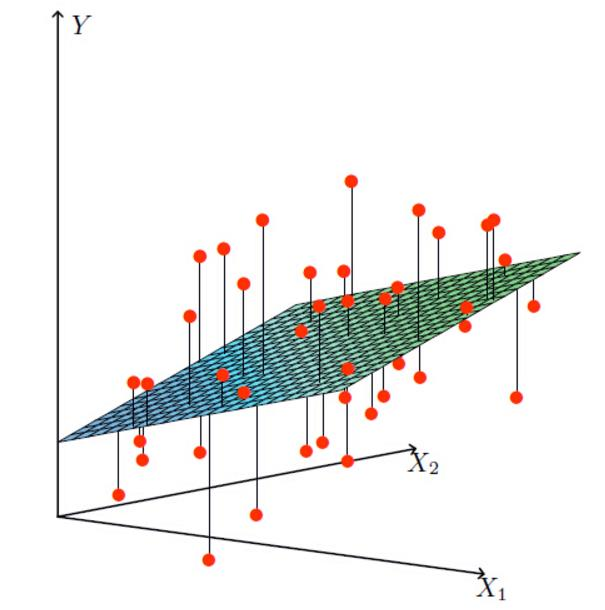
\includegraphics[scale=0.5]{fitting_plane.jpg}
			\renewcommand{\figurename}{Fig} % set picture title starting with Fig or 图
			\caption{fitting plane in sample space}
			\label{fig:1}
		\end{figure}
		the common condition is as section one show, dataset D has d property. at present, it should try to study 
		\begin{equation}f(\boldsymbol x_i) = \boldsymbol{w^{T}}\boldsymbol{x_{i}} + b\end{equation}
		\qquad let \begin{equation}f(\boldsymbol x_i)\cong{y_i}\end{equation}
		\qquad this condition named multivariate linear regression.
		\subsection{\quad analysis}
		similarly, estimate w and b by least square method. 
		conveniently, 
		\begin{equation}\hat{\boldsymbol{w}} = (\boldsymbol{w}; b)\end{equation}
		dataset D show as a matrix $\boldsymbol{X}$, shape $m\times (d+1)$
		\begin{equation}
			\boldsymbol{X}\text{=}
			\left( 
			\begin{matrix}
			{{x}_{11}} & {{x}_{12}} & \cdots  & {{x}_{1d}} & 1  \\
			{{x}_{21}} & {{x}_{22}} & \cdots  & {{x}_{2d}} & 1  \\
			\vdots  & \vdots  & \ddots  & \vdots  & \vdots   \\
			{{x}_{m1}} & {{x}_{m2}} & \cdots  & {{x}_{md}} & 1  \\
			\end{matrix} 
			\right)
			=
			\left( 
			\begin{matrix}
			x_{1}^{T} & 1  \\
			x_{2}^{T} & 1  \\
			\vdots  & \vdots   \\
			x_{m}^{T} & 1  \\
			\end{matrix} 
			\right)
		\end{equation}
		\begin{equation}\text{tag }\boldsymbol{y} = (y_1; y_2; \cdots; y_m)\end{equation}
		so fitting plane \begin{equation}h_w(x) = w_0+w_1x+w_2x+...+w_dx, w_0 
		\text{ is bias}\end{equation}
	
		in summary, \begin{equation}h_w(x) = \sum_{i=0}^{n}w_{i}x_{i} = w^{T}x\end{equation}
	
	\subsection{\quad processing}
	$\boldsymbol \varepsilon$ error, represent the difference between true and predict value.
	
	for every sample, \begin{equation}y^i = w^Tx^i + \varepsilon^i\end{equation}
	\qquad whether $\varepsilon$ obey the independent and identical distribution, and observe mean 0 and var $\theta^2$ distribution.
	
	$\varepsilon$ obey gause distribution, \begin{equation}p(\varepsilon^i) = \frac{1}{\surd{2\pi \sigma}}e\text{x}p(-\frac{(\varepsilon^i)^2}{2\sigma^2})\end{equation}
	substitution equation 16 into equation 17, as following:
	\begin{equation}
	p(y^i|x^i; w) = \frac{1}{\surd{2\pi} \sigma}e\text{x}p(-\frac{(y^i - w^T x^i)^2}{2\sigma^2})
	\end{equation}
	注意, 这里分号后面的 参数 w 仅表示 p依赖于 w 的值, w并不是 p 的前置条件, 而只是这个概率分布的一个参数而已, 也可以省略分号后的内容
	
	likelihood function: % explaintion: the probability every sample belong to real tag is more big and more better.
	\begin{equation}
	L(w) = \underset{i=1}{\overset{m}{\mathop{\prod }}} p(y^i|x^i; w) = \underset{i=1}{\overset{m}{\mathop{\prod }}} \frac{1}{\surd{2\pi} \sigma}e\text{x}p(-\frac{(y^i - w^T x^i)^2}{2\sigma^2})
	\end{equation}
	 
	logarithmic likelihood function: % explaintion: simplify the calculate
	\begin{equation}
		\log{L(w)} = \log{\underset{i=1}{\overset{m}{\mathop{\prod }}} p(y^i|x^i; w) = \underset{i=1}{\overset{m}{\mathop{\prod }}} \frac{1}{\surd{2\pi} \sigma}e\text{x}p(-\frac{(y^i - w^T x^i)^2}{2\sigma^2})}
	\end{equation}
	
	expand equation 20th: 
	% split could show only one tag
	\begin{align}
	\begin{split}
	L(w) &= \sum_{i=1}^{m} \log \frac{1}{\surd{2\pi} \sigma}e\text{x}p(-\frac{(y^i - w^T x^i)^2}{2\sigma^2}) \\
		 &= m\log \frac{1}{\surd{2\pi} \sigma} - \frac{1}{\sigma^2}\cdot \frac{1}{2}\sum_{i=1}^{m}(y^i - w^T x^i)^2
	\end{split}
	\end{align}
	
	target: $L(w)$ more big and more better
	\begin{equation}
	J(w) = \frac{1}{2}\sum_{i=1}^{m}(y^i - w^T x^i)^2\quad\text{(least square method)}
	\end{equation}
	
	target function:
	\begin{align}
		\begin{split}
	J(w) &= \frac{1}{2}\sum_{i=1}^{m}(h_w(x^i) - y^i)^2\\
		 &= \frac{1}{2}(\boldsymbol{X\hat{w}} - \boldsymbol{y})^T(\boldsymbol{X\hat{w}} - \boldsymbol{y})
		 \end{split}
	\end{align}
	
	solve partial derivation:
	\begin{align}
	\begin{split}
    \bigtriangledown_wJ(w) &= \bigtriangledown_w(\frac{1}{2}(\boldsymbol{X\hat{w}} - \boldsymbol{y})^T(\boldsymbol{X\hat{w}} - \boldsymbol{y}))\\
    &= \bigtriangledown_w(\frac{1}{2}(\boldsymbol{\hat{w}^TX^T} - \boldsymbol{y^T})(\boldsymbol{X\hat{w}} - \boldsymbol{y}))\\
    &= \bigtriangledown_w((\frac{1}{2}(\boldsymbol{\hat{w}^TX^TXw} - \boldsymbol{\hat{w}^TX^Ty} - \boldsymbol{yX\hat{w}} + \boldsymbol{y^Ty)})\\
    % matrix derivation
    &= \frac{1}{2}(2\boldsymbol{X^TX\hat{w}} - \boldsymbol{X^Ty} -\boldsymbol{X^Ty})\\
    &= \boldsymbol{X^TX\hat{w}} - \boldsymbol{X^Ty}
	\end{split}
	\end{align}
	
	let partial derivation be equal to 0:
	\begin{equation}
	\boldsymbol{\hat{w}} = \boldsymbol{(X^TX)^{-1}X^Ty}
	\end{equation} 
	
	estimate method:
	original estimate part 
	\begin{equation}
	R^2 = 1-\frac{\sum_{i=1}^{m}(\hat{y}_i - y_i)^2}{\sum_{i=1}^{m}(y_i - \bar{y}_i)^2}
	\end{equation}
	when $R^2$ value is very close approximation to 1, the model fits dataset D well.
	
	\subsection{\quad deep analysis}
	if $X^TX$ is irreversible or avoid over fitting, increase $\lambda$ destabilization
	\begin{equation}
	\theta = (X^TX + \lambda I)^{-1}X^Ty
	\end{equation} 
	
	to remember conclusion simply,
	\begin{align}
		\begin{split}
		X\theta = y \Rightarrow X^TX\theta = X^Ty \Rightarrow \theta = (X^TX)^{-1}X^Ty
		\end{split}
	\end{align}
	
	after add $\lambda$ destabilization:
	\begin{itemize}
		\item $X^TX$ is positive semidefinite matrix: for any non-zero vector u
		\begin{equation}
			\theta X^T X \theta = (X \theta)^T X \theta \overset{define\  v = X \theta}{  \longrightarrow} v^T v \geq 0
		\end{equation}
		\item for any real $\lambda > 0$, $X^T X + \lambda I$ is positive definite matrix, and is reversible. be sure that regerssion equation must be significative.
		\begin{equation}\theta = (X^T X + \lambda I)^{-1} X^T y\end{equation}
	\end{itemize}

	\subsection{\quad penalty factor}
	\begin{itemize}
		\item the target function of linear regerssion:
			\begin{align}
			J(\theta) = \frac{1}{2}\sum_{i=1}^{m}(h_\theta(x^i) - y^i)^2
			\end{align}
		
		\item increase square sum loss:
			\begin{align}
			J(\theta) = \frac{1}{2}\sum_{i=1}^{m}(h_\theta(x^i) - y^i)^2 + \lambda \sum_{j=1}^{m}\theta_{j}^{2}
			\end{align}
			
		\item actually, assume that parameter $\theta$ obey Gaussian distribution
	\end{itemize}

	\subsection{\quad |w|and $|\text{w}|^2$}
	\begin{figure}[H]
		\vspace{-0.2cm}  %调整图片与上文的垂直距离
		\setlength{\abovecaptionskip}{-0.2cm}   %调整图片标题与图距离
		%\setlength{\belowcaptionskip}{0.5cm}   %调整图片标题与下文距离
		\centering
		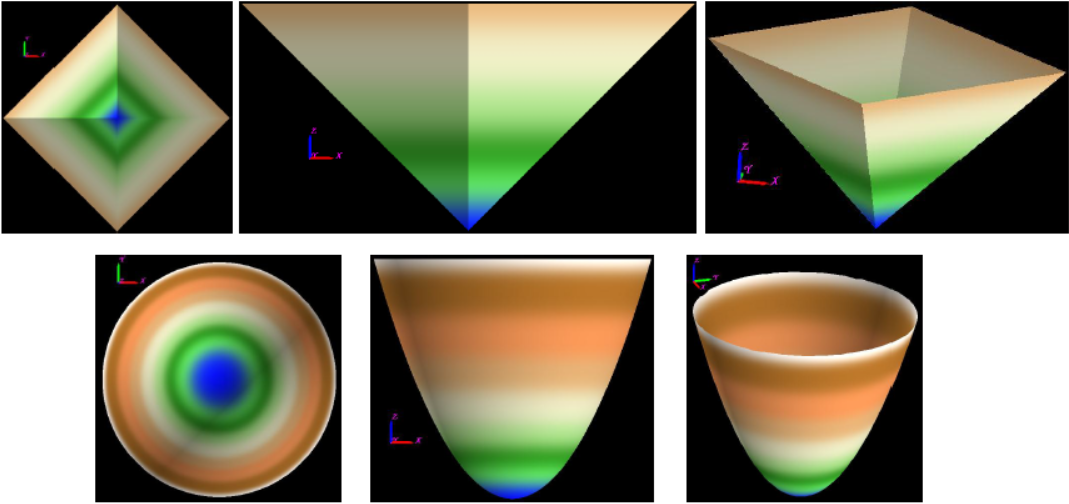
\includegraphics[scale=0.4]{w_and_w^2.png}
		\renewcommand{\figurename}{Fig} % set picture title starting with Fig or 图
		\caption{|w| and $|\text{w}|^2$}
		\label{fig:2}
	\end{figure}
%%%%%%%%%%%%%%%%%%%%%%%%%%%%%%%%%%%%%%%%%%%%%%%%%%%%%%%%%%%%%%%%%%%%%%%%%%%%%%%%%%%%%%%%%%%%%%%
%%%%%%%%%%%%%%%%%%%%%%%%%%%%%%%%%%%%%%%%%%%%%%%%%%%%%%%%%%%%%%%%%%%%%%%%%%%%%%%%%%%%%%%%%%%%%%%
	\section{\quad machine learning and data analysis}
	\begin{figure}[H]
		\vspace{-0.5cm}  %调整图片与上文的垂直距离
		\setlength{\abovecaptionskip}{-0.2cm}   %调整图片标题与图距离
		%\setlength{\belowcaptionskip}{-1cm}   %调整图片标题与下文距离
		\centering
		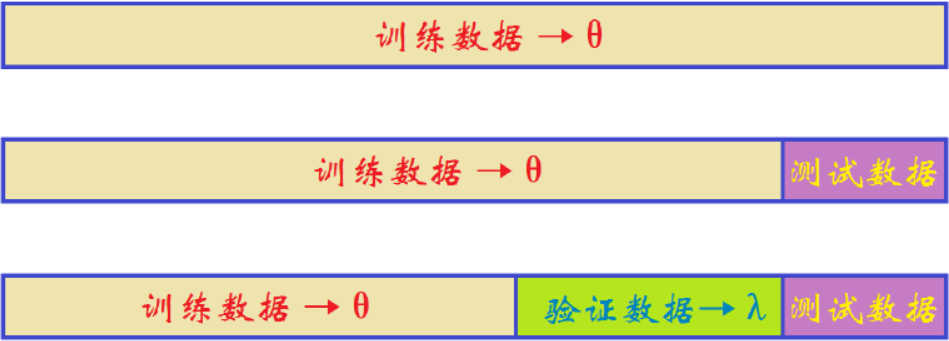
\includegraphics[scale=0.4]{machine_learning_and_data_analysis.png}
		\renewcommand{\figurename}{Fig} % set picture title starting with Fig or 图
		\caption{machine learning and data analysis}
		\label{fig:3}
	\end{figure}
	\begin{itemize}
		\item cross validation:
		\subitem example: 10 folk cross validation
	\end{itemize}

	\section{ conclusion}
		\subsection{\quad probability and statistics}
			概率(probabilty)和统计(statistics)看似两个相近的概念,其实研究的问题刚好相反。
			
			
			概率研究的问题是,已知一个模型和参数,怎么去预测这个模型产生的结果的特性(例如均值,方差,协方差等等)。 举个例子,我想研究怎么养猪(模型是猪),我选好了想养的品种、喂养方式、猪棚的设计等等(选择参数),我想知道我养出来的猪大概能有多肥,肉质怎么样(预测结果)。
			
			
			统计研究的问题则相反。统计是,有一堆数据,要利用这堆数据去预测模型和参数。仍以猪为例。现在我买到了一堆肉,通过观察和判断,我确定这是猪肉(这就确定了模型。在实际研究中,也是通过观察数据推测模型是/像高斯分布的、指数分布的、拉普拉斯分布的等等),然后,可以进一步研究,判定这猪的品种、这是圈养猪还是跑山猪还是网易猪,等等(推测模型参数)。
			
			
			一句话总结:概率是已知模型和参数,推数据。统计是已知数据,推模型和参数。 
			
			
			显然,对于最大似然估计,最大后验估计,贝叶斯估计来说,都属于统计的范畴。
		
		\subsection{theory of MLE}
			目的: 利用已知的样本结果,反推最有可能(最大概率)导致这样结果的参数值
			
			 原理:极大似然估计是建立在极大似然原理的基础上的一个统计方法,是概率论在统计学中的应用。极大似然估计提供了一种给定观察数据来评估模型参数的方法,即:“模型已定,参数未知”。通过若干次试验,观察其结果,利用试验结果得到某个参数值能够使样本出现的概率为最大,则称为极大似然估计。
			 
		\subsection{\quad likelihood and probability}
			在非正式场合似然和概率 Probability 几乎是一对同义词,但是在统计学中似然和概率却是两个不同的概念。
			
			概率是在特定环境下某件事情发生的可能性,也就是结果没有产生之前依据环境所对应的参数来预测某件事情发生的可能性,比如抛硬币,抛之前我们不知道最后是哪一面朝上,但是根据硬币的性质我们可以推测任何一面朝上的可能性均为50\%,这个概率只有在抛硬币之前才是有意义的,抛完硬币后的结果便是确定的;
			
			而似然刚好相反,是在确定的结果下去推测产生这个结果的可能环境(参数),
			
			还是抛硬币的例子,假设我们随机抛掷一枚硬币1,000次,结果500次人头朝上,500次数字朝上(实际情况一般不会这么理想,这里只是举个例子),我们很容易判断这是一枚标准的硬币,两面朝上的概率均为50\%,这个过程就是我们根据结果来判断这个事情本身的性质(参数),也就是似然。
			
		\subsection{\quad representation}
			结果和参数相互对应的时候,似然和概率在数值上是相等的,如果用 $\theta$ 表示环境对应的参数,x 表示结果,那么概率可以表示为:
				$$P(x|\theta)$$
			是条件概率的表示方法,$\theta$ 是前置条件,理解为在 $\theta$ 的前提下,事件 x 发生的概率,相对应的似然可以表示为:
				$$L(\theta|x)$$
			理解为已知结果为 x ,参数为 $\theta$ (似然函数里 $\theta$  是变量,这里说的参数是相对与概率而言的)对应的概率,即:
			$$L(\theta|x) = P(x|\theta)$$
			需要说明的是两者在数值上相等,但是意义并不相同,$$L(\theta|x)$$ 是关于 $\theta$ 的函数,而 P 则是关于 x 的函数,两者从不同的角度描述一件事情。
			
	\section{\quad least square method vs maximum likelihood estimate}
		\subsection{\quad difference}
			对于最小二乘法,当从模型总体随机抽取n组样本观测值后,最合理的参数估计量应该使模型最好地拟合样本数据,也就是使估计值和观测值之差的平方和最小。而对于最大似然法,当从模型中随机抽取n组样本观测值之后,最合理的参数估计量应该使得从模型中抽取的该n组样本观测值的概率最大。显然,这是从不同的原理出发的两种参数估计方法。
			
		\subsection{\quad the similarity}
			在最大似然法中,通过选择参数,使已知数据在某种意义下最有可能出现,而某种意义通常指似然函数最大,而似然函数又往往指数据的概率分布函数。与最小二乘法不同的是,最大似然法需要已知这个概率分布函数,这在实践中是很困难的。
			\textcolor{red}{一般假设其满足正态分布函数的特性,在这种情况下,最大似然估计和最小二乘估计相同}. 最小二乘法以估计值与观测值的差的平方和作为损失函数,极大似然法则是以最大化目标值的似然概率函数为目标函数,从概率统计的角度处理线性回归并在似然概率函数为高斯函数的假设下同最小二乘建立了的联系
		
	\section{\quad MAP}
		\subsection{\quad concept}
			最大似然估计是求参数$\theta$, 使似然函数$P(x_0|\theta)$最大。最大后验概率估计则是想求$\theta$使$P(x_0|\theta)P(\theta)$最大。求得的$\theta$不单单让似然函数大,$\theta$自己出现的先验概率也得大。(这有点像正则化里加惩罚项的思想,不过正则化里是利用加法,而MAP里是利用乘法)
		
		\subsection{\quad theory}
			MAP其实是在最大化
			$P(\theta|x_0)=\frac{P(x_0 \theta) P(\theta)}{P(x_0)}$
			,不过因为 $x_0$ 是确定的(即投出的“反正正正正反正正正反”),$P(x_0)$是一个已知值,所以去掉了分母 $P(x_0)$ (假设“投10次硬币”是一次实验,实验做了1000次,“反正正正正反正正正反”出现了n次,则$P(x_0)=n/1000$。总之,这是一个可以由数据集得到的值)。最大化$P(\theta|x_0)$的意义也很明确,$x_0$已经出现了,要求 $\theta$ 取什么值使 $P(\theta|x_0)$ 最大。顺带一提,$P(\theta|x_0)$ 即后验概率,这就是“最大后验概率估计”名字的由来。

		\subsection{\quad $P(\theta)$ value}
			$P(\theta)$ 实际中是用的 $\theta$ 的概率密度函数描述的。因为在式子里面它使用的在 $\theta$ 这个点处的概率,但是由于 $\theta$ 可以看作是一个连续随机变量,所以某个点处的概率可能直接无法得到一个函数来描述。但是利用概率密度函数可以达到同样的效果,因为每个点出的概率可以看作是概率函数每个点对应的小矩形条的面积,所以其实和乘上每个 $\theta$ 值处的概率效果是一样
		
		\subsection{\quad analysis}
			对于投硬币的例子来看,我们认为(先验地知道) $\theta$ 取0.5的概率很大,取其他值的概率小一些。我们用一个高斯分布来具体描述我们掌握的这个先验知识,例如假设 $P(\theta)$为均值0.5,方差0.1的高斯函数,如下图:
				\begin{figure}[H]
					\vspace{-0.5cm}  %调整图片与上文的垂直距离
					\setlength{\abovecaptionskip}{-0.2cm}   %调整图片标题与图距离
					%\setlength{\belowcaptionskip}{-1cm}   %调整图片标题与下文距离
					\centering
					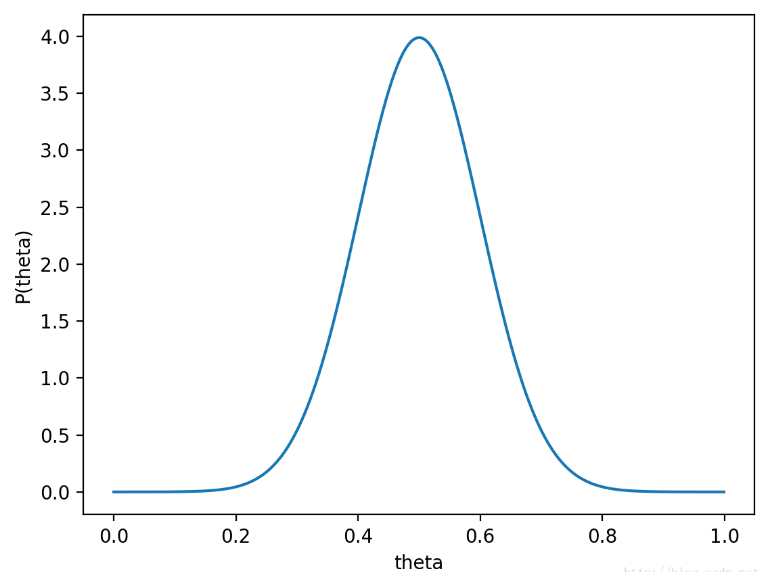
\includegraphics[scale=0.4]{gussian_distribution.png}
					\renewcommand{\figurename}{Fig} % set picture title starting with Fig or 图
					\caption{gussian distribution}
					\label{fig:4}
				\end{figure}
			则 $P(x_0|\theta) P(\theta)$ 的函数图像为($(1-\theta)^3*\theta^7*e^{(-100(\theta-0.5)^2)}$)
				\begin{figure}[H]
					\vspace{-0.5cm}  %调整图片与上文的垂直距离
					\setlength{\abovecaptionskip}{-0.2cm}   %调整图片标题与图距离
					%\setlength{\belowcaptionskip}{-1cm}   %调整图片标题与下文距离
					\centering
					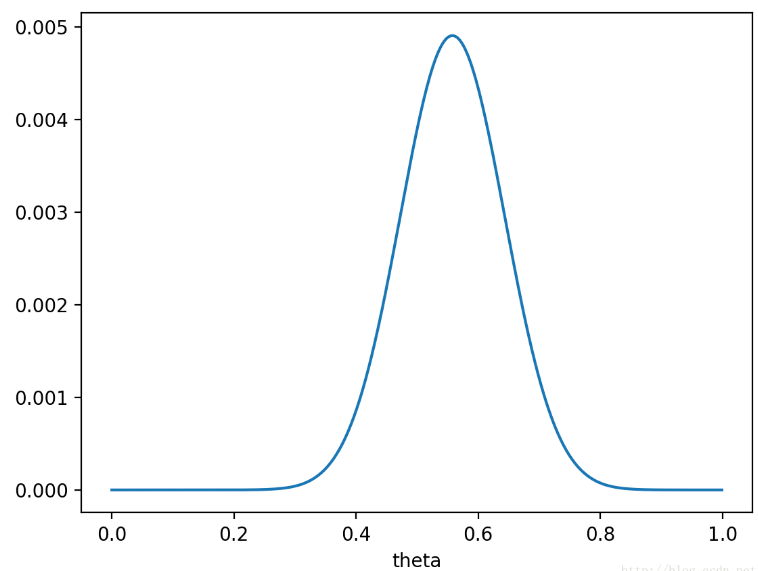
\includegraphics[scale=0.4]{MAP_gussian_distribution.png}
					\renewcommand{\figurename}{Fig} % set picture title starting with Fig or 图
					\caption{MAP gussian distribution}
					\label{fig:5}
				\end{figure}
			注意,此时函数取最大值时,$\theta$ 取值已向左偏移,不再是0.7。实际上,在 $\theta=0.558$ 时函数取得了最大值。即,用最大后验概率估计,得到 $\theta=0.558$
			\\
			最后,那要怎样才能说服一个贝叶斯派相信 $\theta=0.7$呢?你得多做点实验。
			\\
			如果做了1000次实验,其中700次都是正面向上,这时似然函数为:
					\begin{figure}[H]
						\vspace{-0.5cm}  %调整图片与上文的垂直距离
						\setlength{\abovecaptionskip}{-0.2cm}   %调整图片标题与图距离
						%\setlength{\belowcaptionskip}{-1cm}   %调整图片标题与下文距离
						\centering
						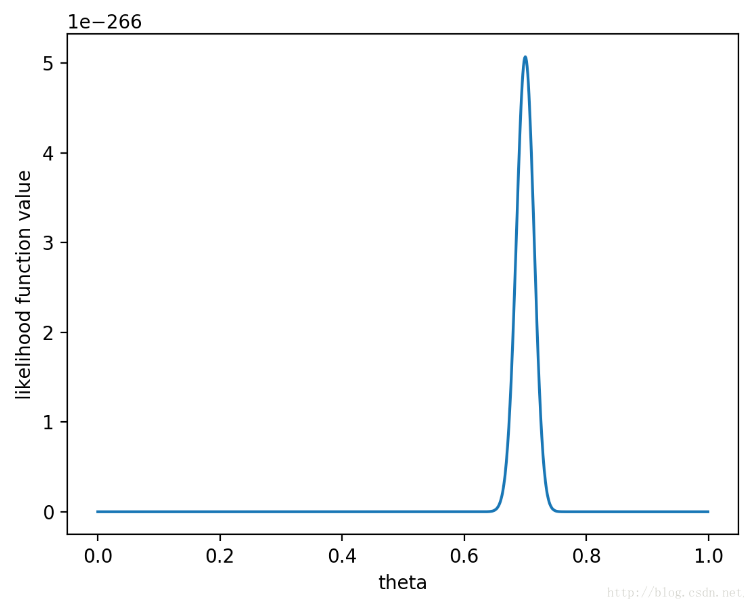
\includegraphics[scale=0.4]{likelihood_function_gussian_distribution.png}
						\renewcommand{\figurename}{Fig} % set picture title starting with Fig or 图
						\caption{likelihood function gussian distribution}
						\label{fig:6}
					\end{figure}
			如果仍然假设 $P(\theta)$ 为均值0.5,方差0.1的高斯函数,$P(x_0|\theta)P(\theta)$的函数图像为:
					\begin{figure}[H]
						\vspace{-0.5cm}  %调整图片与上文的垂直距离
						\setlength{\abovecaptionskip}{-0.2cm}   %调整图片标题与图距离
						%\setlength{\belowcaptionskip}{-1cm}   %调整图片标题与下文距离
						\centering
						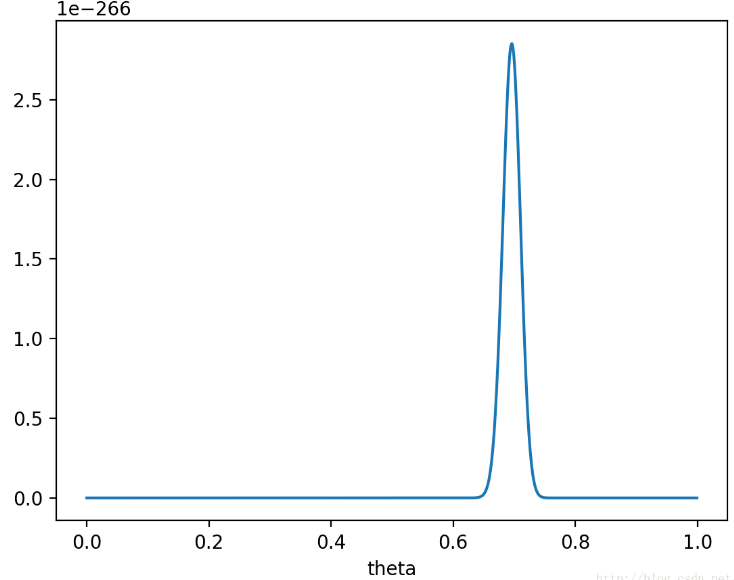
\includegraphics[scale=0.4]{big_sample_MAP_gussian_distribution.png}
						\renewcommand{\figurename}{Fig} % set picture title starting with Fig or 图
						\caption{big sample MAP gussian distribution}
						\label{fig:7}
					\end{figure}
			在 $\theta=0.696$ 处,$P(x_0|\theta)P(\theta)$取得最大值。
			
			这样,就算一个考虑了先验概率的贝叶斯派,也不得不承认得把 $\theta$ 估计在0.7附近了。
			
			PS. 要是遇上了顽固的贝叶斯派,认为 $P(\theta=0.5)=1$ ,那就没得玩了。。 无论怎么做实验,使用MAP估计出来都是 $\theta=0.5$ 。这也说明,一个合理的先验概率假设是很重要的。 (通常,先验概率能从数据中直接分析得到)
	
	\section{\quad the difference between MLE and MAP}
		\begin{itemize}
			\item 	MAP就是多了一个作为因子的先验概率 $P(\theta)$
			
			\item 	MLE可以看做MAP的一个特例,它把先验概率分布看做均匀分布,所以 $P(\theta)$ 是常数,因此 $P(\theta)$ 就不用出现在目标函数里了。
			
			\item 可以认为$P(\theta)$是个均匀分布,处处相等。均匀分布的物理意义是,我们对$\theta$的分布没有任何先验的知识
		\end{itemize}
	
	\section{\quad 理清MLE和Bayes中 $L(\theta|D), P(D|\theta), P(\theta|D), P(D), P(\theta)$}
			\begin{enumerate}
				\item 似然函数: $L(\theta|D)$ 
				
				\item 其定义表示根据给定数据, 找到一个概率最大(即使数据发生可能最大)的参数  $L(\theta|D) = P(D|\theta) = P(x_1, x_2, x_3...,x_n|\theta) = \prod\limits_{k=1}^{n}(x_k|\theta)$ (此处假设样本之间相互独立)
				
				\item $P(\theta|D)$ 表示后验概率,指掌握了一定量的数据后我们的参数分布是怎么样的
				
				\item $P(\theta)$ 表示先验概率,指在没有掌握数据后我们的参数怎么分布
				
				\item $P(D)$ 为数据分布
				
				\item $P(\theta)$ 为先验概率
			\end{enumerate}
		
	\section{\quad the blob about MLE and Bayed}
		\url{https://blog.csdn.net/liu1194397014/article/details/52766760}		
		\par
		\begin{enumerate}
			\item[]
				\begin{figure}[H]
					%\label{margin}
					\vspace{-0.2cm}  %调整图片与上文的垂直距离
					%\setlength{\abovecaptionskip}{-0.2cm}   %调整图片标题与图距离
					%\setlength{\belowcaptionskip}{-1cm}   %调整图片标题与下文距离
					\centering
					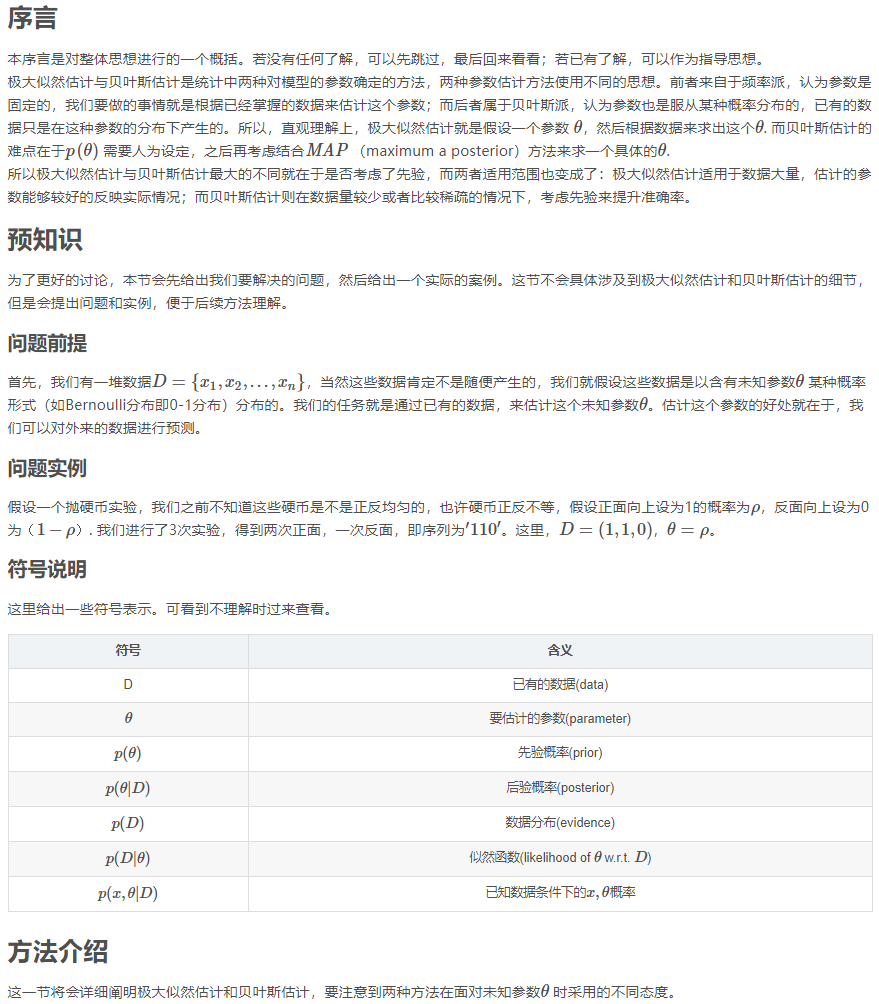
\includegraphics[scale=0.8]{MLE_and_Bayes.png}
					\renewcommand{\figurename}{Fig} % set picture title starting with Fig or 图
					%\caption{functional margin and geometric margin}
				\end{figure}
			
			\item[] 
				\begin{figure}[H]
					%\label{margin}
					\vspace{-0.2cm}  %调整图片与上文的垂直距离
					%\setlength{\abovecaptionskip}{-0.2cm}   %调整图片标题与图距离
					%\setlength{\belowcaptionskip}{-1cm}   %调整图片标题与下文距离
					\centering
					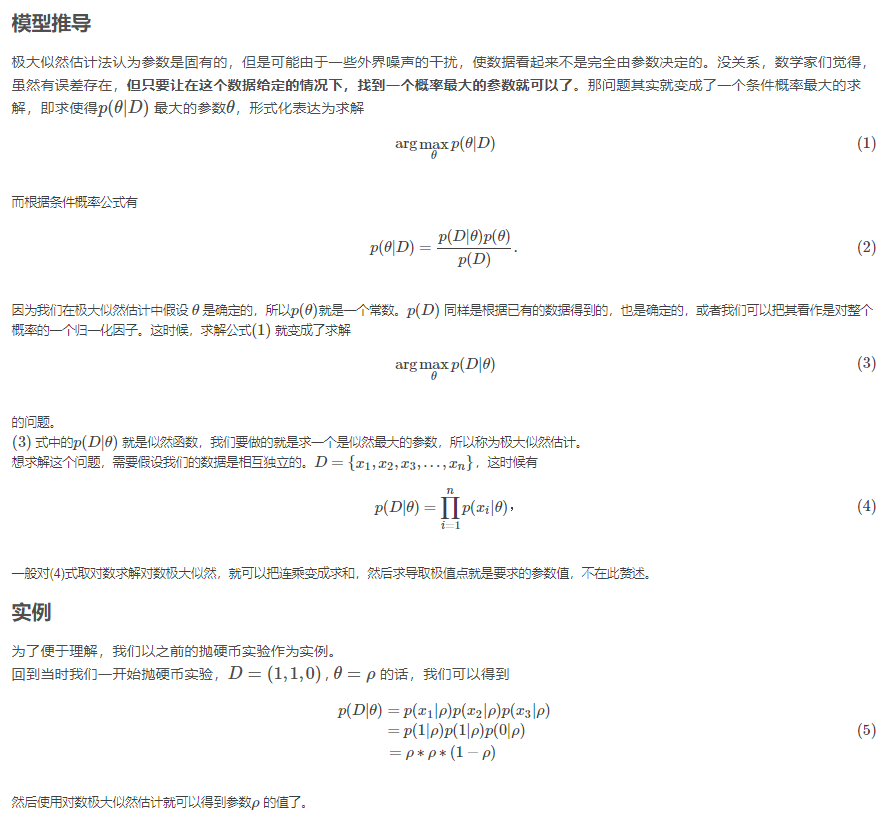
\includegraphics[scale=0.8]{derivation_MLE.png}
					\renewcommand{\figurename}{Fig} % set picture title starting 
				\end{figure}
			
			\item[] 
				\begin{figure}[H]
					%\label{margin}
					\vspace{-0.2cm}  %调整图片与上文的垂直距离
					%\setlength{\abovecaptionskip}{-0.2cm}   %调整图片标题与图距离
					%\setlength{\belowcaptionskip}{-1cm}   %调整图片标题与下文距离
					\centering
					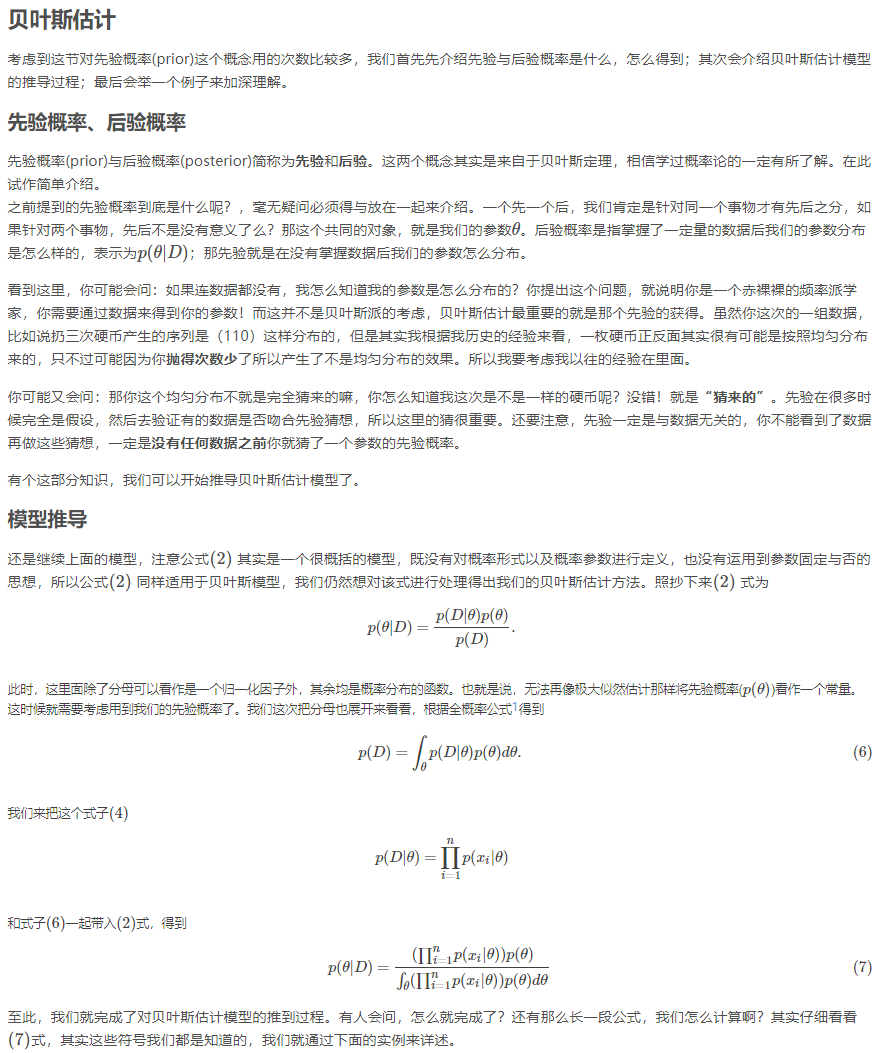
\includegraphics[scale=0.8]{derivation_bayes.png}
					\renewcommand{\figurename}{Fig} % set picture title starting with Fig or 图
				\end{figure}
			
			\item[] 
				\begin{figure}[H]
					%\label{margin}
					\vspace{-0.2cm}  %调整图片与上文的垂直距离
					%\setlength{\abovecaptionskip}{-0.2cm}   %调整图片标题与图距离
					%\setlength{\belowcaptionskip}{-1cm}   %调整图片标题与下文距离
					\centering
					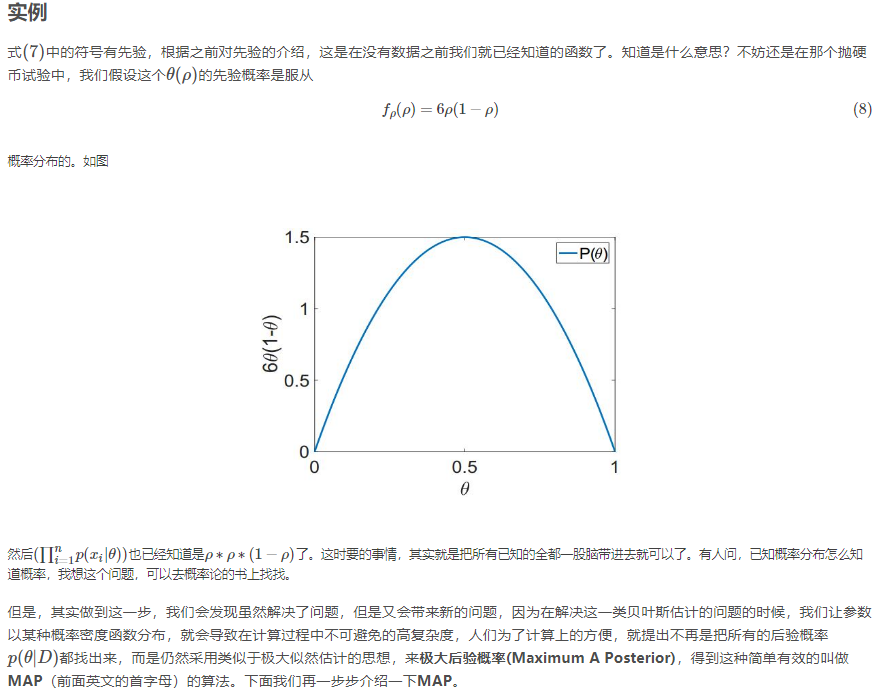
\includegraphics[scale=0.8]{example_bayes.png}
					\renewcommand{\figurename}{Fig} % set picture title starting 
				\end{figure}
			
			\item[] 
				\begin{figure}[H]
					%\label{margin}
					\vspace{-0.2cm}  %调整图片与上文的垂直距离
					%\setlength{\abovecaptionskip}{-0.2cm}   %调整图片标题与图距离
					%\setlength{\belowcaptionskip}{-1cm}   %调整图片标题与下文距离
					\centering
					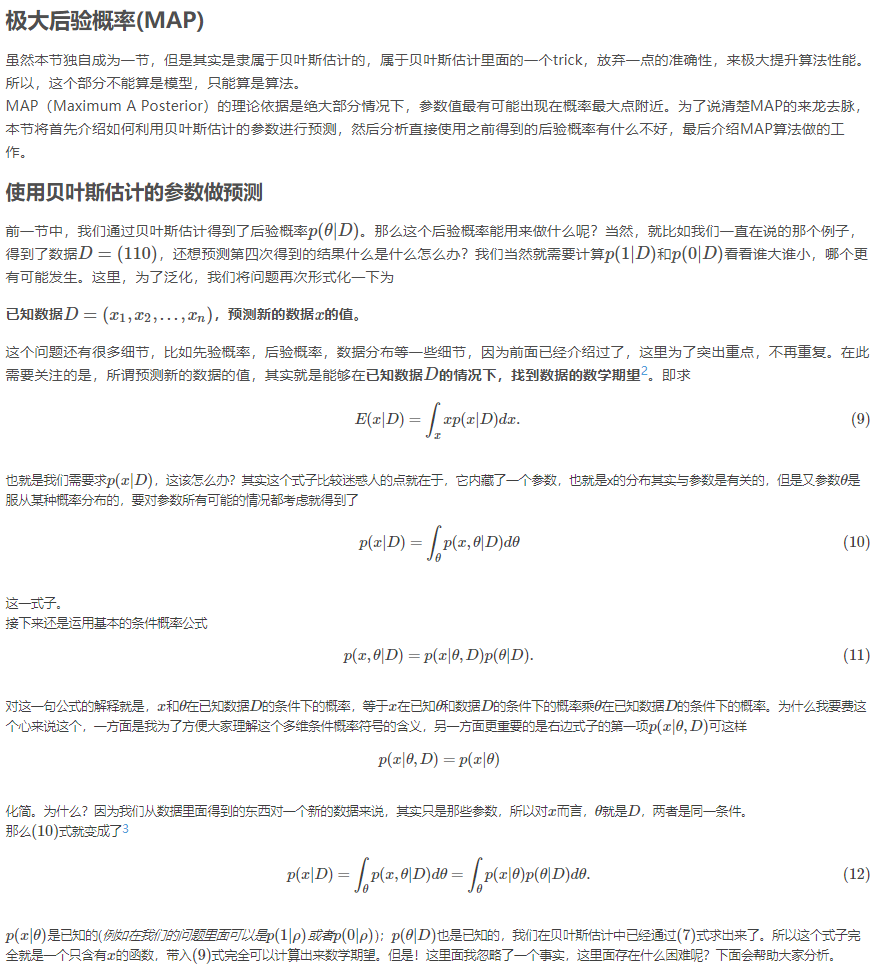
\includegraphics[scale=0.8]{derivation_MAP.png}
					\renewcommand{\figurename}{Fig} % set picture title starting with Fig or 图
				\end{figure}
			
			\item[] 
				\begin{figure}[H]	
					\vspace{-0.2cm}  %调整图片与上文的垂直距离
					%\setlength{\abovecaptionskip}{-0.2cm}   %调整图片标题与图距离
					%\setlength{\belowcaptionskip}{-1cm}   %调整图片标题与下文距离
					\centering
					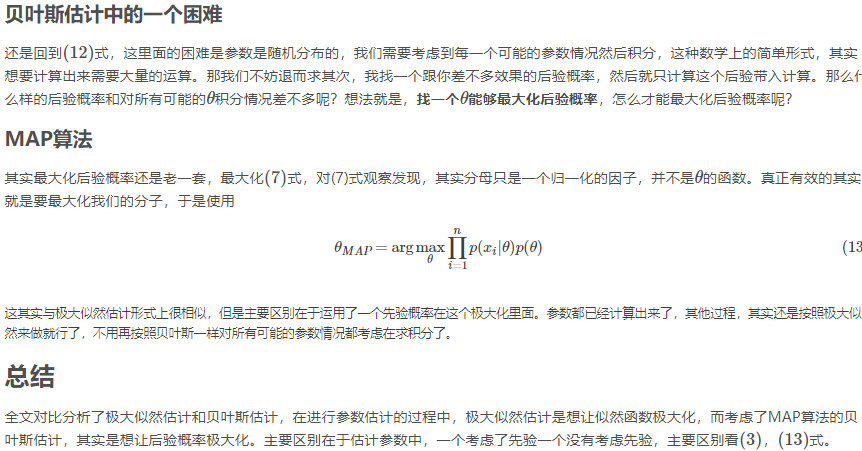
\includegraphics[scale=0.8]{conclusion_MLE_and_Bayes.png}
					\renewcommand{\figurename}{Fig} % set picture title starting with Fig or 图
					\caption{极大似然估计与贝叶斯估计}
					\label{fig:blob}
				\end{figure}	
		\end{enumerate}		
			
	
		
	\section{\quad reference}
		\subsection{\quad the relationship and difference between MLE、MAP、Bayse estimate}
			\url{https://blog.csdn.net/bitcarmanlee/article/details/81417151}
			
		\subsection{\quad detail of MLE and MAP}
			\url{https://www.cnblogs.com/sylvanas2012/p/5058065.html}
			
		\subsection{\quad least square and gradient descend and maximum likelihood}
			\url{https://blog.csdn.net/FrankieHello/article/details/81432769}
			
		\subsection{\quad detail of MLE}
			\url{https://blog.csdn.net/u014182497/article/details/82252456}
			
		\subsection{\quad understand deeply MLE and MAP}
			\url{https://blog.csdn.net/u011508640/article/details/72815981}
		
		\subsection{\quad difference between Bayes and MLE}
		\url{https://blog.csdn.net/feilong_csdn/article/details/61633180}
\end{document}

